\chapter{Implementation}
\label{chap:Implementation}
In this chapter we explain the infrastructure that performs all the necessary steps to produce an efficient feedback. A general overview is given and for each section, we describe in particular the tools as well as the way we manipulated the data in order to obtain the information useful for the user. The chapter is divided in two parts: the first part focuses on the back-end and the services we used to extract the features we described in \ref{chap:Speech Recognition}. The second part describe the front-end, that is, the \textit{Android}\footnote{\url{https://www.android.com}} application (called \textbf{PARLA}\footnote{\url{https://github.com/davideberdin/PARLA}}) with a particular focus on the feedback page and the general usage.

\section{General architecture}
\label{sec:general_architecture}

In \ref{fig:general_architecture} is shown the general architecture of the infrastructure.
The flow displays only the \textit{pronunciation testing} phase:

\begin{itemize}
	\item[1)] User says the sentence using the internal microphone of the smartphone (or through the headset)
	\item[2)] The application sends the audio file to the \textit{Speech Recognition service}
	\item[3)] The result of step 2 is sent to the \textit{Gaussian Mixture Model service}
	\item[4)] The result of step 3 is sent back to the application where a \textit{Feedback page} is displayed
	\item[5)] A short explanation for each chart is given to the user
	\item[6)] Back to step 1
\end{itemize}

\begin{figure}[!ht]
	\centering
	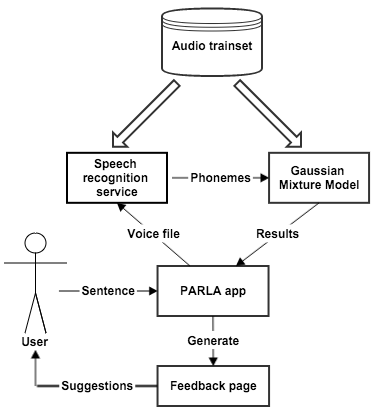
\includegraphics[scale=0.6]{Figures/general_architecture.png}
	\caption{General architecture of the infrastructure}
	\label{fig:general_architecture}
\end{figure}


\section{Server}
\label{sec:server}

\begin{figure}[!ht]
	\centering
	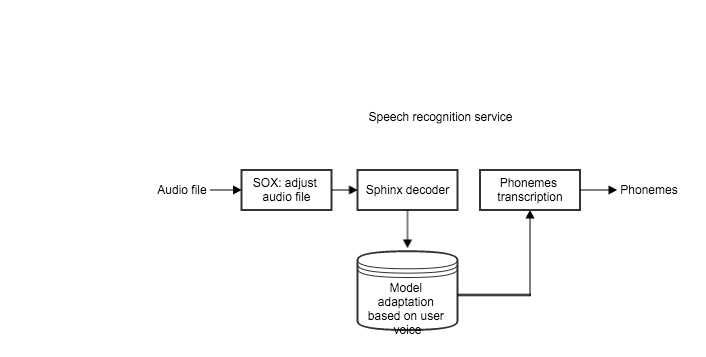
\includegraphics[scale=0.6]{Figures/sphinx_service.png}
	\caption{Architecture of the Speech recognition service}
	\label{fig:sphinx_service}
\end{figure}

\begin{figure}[!ht]
	\centering
	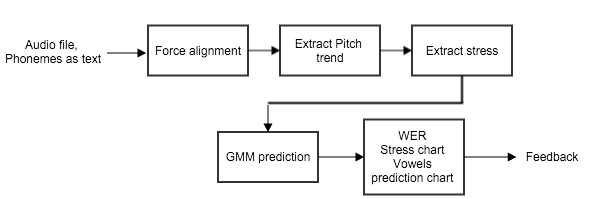
\includegraphics[scale=0.6]{Figures/gmm_service.png}
	\caption{Architecture of the Gaussian Mixture Model service}
	\label{fig:gmm_service}
\end{figure}

\section{Data collection}
\label{sec:data_collection}

\subsection{Data pre-processing}
\label{ssec:pre_processing}


\subsection{Training the Speech Recognition model} 
\label{ssec:training_sr_model}


\subsection{Training the Gaussian Mixture Model}
\label{ssec:training_gmm}

- BIC, AIC and other things here


%%%%%%%%%%%%%%%%%%%%%%%%%%%%%%%%%%%%%%%%%%%%%%%%%%%%%%%%%%%%%%%%%%%%%%%%%%%%%%%%
%%%%%							ANDROID PART							   %%%%%
%%%%%%%%%%%%%%%%%%%%%%%%%%%%%%%%%%%%%%%%%%%%%%%%%%%%%%%%%%%%%%%%%%%%%%%%%%%%%%%%


\section{Android application}
\label{sec:android_app}

\subsection{Layouts}
\label{ssec:layouts}

\subsection{Feedback layout}
\label{ssec:feedback_layout}

\subsection{Usage procedure}
\label{ssec:usage_procedure}